\chapter{Preliminaries}

%Gröbnerbasen, Buchberger

% Keine Schemata, alles affine Varietäten
% K algebraisch abgeschlossen, alle Varietäten sind über k

\section{Algebraic group actions}

In this section we extend the notion of groups acting on sets to actions on objects in algebraic geometry. We only cover the case of affine varieties here. For a more general approach considering pre\=/schemes, see \cite{git}. Broadly speaking, we require the the group and the set operated on to carry structures of affine varieties such that the set\=/theoretical group action becomes a morphism.

\begin{defi}[Actions of affine algebraic groups]
	An \emph{affine algebraic group} $G$ is an affine variety together with a morphism $m\colon G \times G \rightarrow G$ such that $G$ carries a group structure with the group law $m$. A \emph{homomorphism} of algebraic groups $G$ and $H$ is a morphism $f\colon G \rightarrow H$ such that $f$ preserves the group structure.
\end{defi}

\begin{ex}
	The affine variety $$(\field^*)^n \cong V(t_1t_1^{-1} - 1,\dots, t_nt_n^{-1}-1)\subseteq\field[t_1,t_1^{-1},...,t_n,t_n^{-1}]$$
	is an affine algebraic group via the group law
	$$m\colon (\field^*)^n \times (\field^*)^n \rightarrow (\field^*)^n,\quad ((r_1,\dots,r_n),(s_1,\dots,s_n)) \mapsto (r_1s_1,\dots,r_ns_n).$$
	Note that $m$ is polynomial when formulated over $\field[t_1,t_1^{-1},...,t_n,t_n^{-1}]$.
\end{ex}

\begin{defi}
	An affine algebraic group $G$ is called \emph{(algebraic) torus of dimension $n$} iff there exists $n>0$ such that $G$ is isomorphic to the affine algebraic group $(\field^*)^n$.
\end{defi}

\begin{remark}
	\label{remark:torus_from_integral_vectors}
	Let $\field$ be a algebraically closed field of characteristic zero. Then any finite set $\{v_1,\dots,v_r\}\subseteq\integer^k$ of integral vectors constitutes an algebraic torus of the same dimension as the linear subspace $L = \langle v_1,\dots,v_r\rangle_\rational$. Denote the dimension of $L$ by $d$. Then there exists an $\rational$-linear isomorphism such that $L\cong \rational^d$. In particular, this isomorphism translates to a $\field$\=/algebra isomorphism $\field[L] \cong \field[\rational^d]$ when $\rational$ is embedded into $\field$ as its prime field.
	It follows that $\spec(\field[L])$ is an algebraic torus via
	$$\spec(\field[L]) \cong \spec(\field[\rational^d]) =(\field^*)^d.$$
\end{remark}

\begin{defi}[Algebraic Group action]
	Let $G$ be an affine algebraic group and $X$ be an affine variety. An (algebraic) group action of $G$ on $X$, denoted by $G\acts X$, is a morphism $\varphi\colon G\times X \rightarrow X$ such that $\varphi$ defines a set\=/theoretic group action of $G$ on $X$ via
	$$g\cdot x \defeq \varphi(g,x).$$
\end{defi}

\begin{ex}
	\label{example:torus_group_action}
	Let $X = V(\ideal)\subseteq\field[x_1,\dots,x_r]$ be an affine variety such that its coordinate ring permits a $\integer^k$\=/grading. This grading extends to a $\integer^k$\=/grading of $\field[\mathbf{x}]$  via
	$$\deg(x_i) \defeq \deg(\overline{x_i})\quad 1\leq i \leq r$$
	so that $\ideal$ becomes homogeneous. The map
	$$*\colon(\field^*)^k \times X \rightarrow X,\quad (t,P) \mapsto (t^{q_1}P_1,\dots,t^{q_r}P_r)$$
	defines a group action. Clearly, the function is polynomial and the identity and compatibility axioms hold. It remains to check that it is well defined. Since we have $f(t*P) = t^q f(P)$ for all homogeneous polynomials $f$ of degree $q\in\integer^k$, for any point $P$ vanishing on the homogeneous ideal $\ideal$, $t*P$ also vanishes on $\ideal$.
\end{ex}

\begin{remark}
	Let $G$ be an affine algebraic group acting on an affine variety $X$. Let $x\in X$. The stabiliser subgroup $G_x$ is a closed, affine subvariety since it is the locus of $I(X)$ and the components of $g\mapsto gx - x$. It follows that $G_x$ is an affine algebraic subgroup.
\end{remark}

\begin{remark}[Group action on regular functions]
	If $\varphi$ is a group action of an affine algebraic group $G$ on an affine variety $X$, we obtain a group action of $G$ on the regular functions $K(X)$ of $X$ by
	$$G\times K(X)\rightarrow K(X), \quad(g,\frac{f}{g}) \mapsto \frac{f\circ \varphi(g^{-1},\wildcard)}{g\circ \varphi(g^{-1},\wildcard)}\ .$$
	
	If $U$ is a $G$\=/invariant open subset of $X$, that is $GU = G$, the restriction of $G\acts K(X)$ to $\O_X(U)$ yields a group action $G\acts\O_X(U)$. Note that if the denominator $g$ does not vanish on any point in $U$, then the same holds for $g\circ \varphi(g^{-1},\wildcard)$ as we have $$\varphi(g^{-1},\wildcard)(U) \subseteq GU = U.$$
	
	We say that $f\in\O_X(U)$ is \emph{$G$\=/invariant} iff $gf = f$ holds for all $g\in G$. The subalgebra of $G$\=/invariant functions is denoted by $\O_X(U)^G$.
	\index{OXUG@$\O_X(U)^G$}%
\end{remark}

\section{Good quotients}
When an algebraic group $G$ acts on an affine variety $X$, naturally one questions if the orbit space $X/G$ defined by the group action can be equipped with the structure of an variety such that the quotient map $p\colon X\rightarrow X/G$ becomes a morphism. Consider the following example.

\begin{ex}
	\label{example:bad_quotient}
	Let $G=\complex^*$ be a one dimensional algebraic torus action on the affine variety $X = \complex^2$ via scaling, that is
	$$(t,(x_1,x_2)) \mapsto (tx_1,tx_2).$$
	Each line $l$ through the origin in $\complex^2$ yields an orbit when removing 0. The origin point is $G$\=/invariant and thus an orbit on its own.
	If the set\=/theoretical quotient map $p$ would be a morphism, a regular function $\varphi$ in $\O(X/G)$ induces a regular function $\psi = \varphi \circ p$ in $\O(X)$ that is $G$\=/invariant. In particular, $\psi$ has to be constant on the closure of each orbit. Since each closure contains the origin, $\psi$ and thus $\varphi$ have to be constant. It follows that $\O(X/G) \cong \field$, contradicting $|X/G| > 1$. Consequently, the set\=/theoretical quotient map is no good quotient in the following sense.
\end{ex}

\begin{defi}[Good quotient, \phantom{}{\cite[Definition 5.0.5]{cls}}]
	Let $G$ be an affine algebraic group acting on an affine variety $X$. A $G$\=/invariant morphism $p\colon X \rightarrow Y$ is called a \emph{good (categorial) quotient}, if
	\begin{enumerate}[label={\upshape(\roman*)}]
		\item the pullback $p^*\colon \O_Y \rightarrow (p^*\O_X)^G$ is an isomorphism of sheaves, that is, for any open $U\subseteq X$ the pullback $p^*\colon \O_Y(U) \rightarrow \O_X(p^{-1}(U))^G$ is an isomorphism of $\field$\=/algebras, (note that preimages of $p$ are $G$\=/invariant)
		\item $p(W)$ is closed for any $G$\=/invariant, closed $W\subseteq X$,
		\item the images of disjoint $G$\=/invariant, closed subsets are disjoint.
	\end{enumerate}
\end{defi}

If $\O(X)^G$ is finitely generated, the canonical embedding $\O(X)^G \hookrightarrow \O(X)$ yields a good quotient $p\colon X \rightarrow Y$, where $Y$ is the affine variety with coordinate ring $\O(X)^G$. The question of $\O(X)^G$ being finitely generated is addressed by Hilbert's fourteenth problem and has been answered negatively by Nagata. \cite[chapter 4]{lectures_invariant_theory}

Good quotients admit the following useful properties.

\begin{prop}[\phantom{}{\cite[Theorem 5.0.6 \& Proposition 5.0.7]{cls}}]
	\label{prop:good_quotient_properties}
	Let $G, X$ be as above. Let $p\colon X \rightarrow Y$ be a good quotient. Then it holds that
	\begin{enumerate}[label={\upshape(\roman*)}]
		\item $p$ is surjective,
		\item for any $G$\=/invariant morphism $\varphi\colon X \rightarrow Z$, there exists a unique morphism $\psi\colon Y \rightarrow Z$ such that $\varphi = \psi \circ p$,
		\label{enum_item:good_quotient_universal_property}
		\item the topology on $Y$ coincides with the quotient topology induced by $p$,
		\item $p$ separates closed $G$\=/orbits, that is
		$$p(x) \neq p(y)\ \Leftrightarrow\ \overline{Gx}\cap\overline{Gy} = \emptyset$$
		for all points $x,y\in X$.
		\item Each fibre of $p$ contains a unique closed G\=/orbit. In particular, $p$ induces a bijection
		$$\{Gx\mid x\in X\ \mathrm{such}\ \mathrm{that}\ Gx = \overline{Gx}\}\simeq Y.$$
		\label{enum_item:good_quotient_space_bijection_closed_orbits}
	\end{enumerate}
\end{prop}

Indeed, good quotients are categorical quotients by \ref{enum_item:good_quotient_universal_property} and the good quotient space $Y$ is unique up to isomorphism. For this reason we also write $X\sslash G$ for $Y$.
\index{X//G@$X\sslash G$}%
Note that by \ref{enum_item:good_quotient_space_bijection_closed_orbits}, in general $X\sslash G$ does not coincide with the orbit space $X / G$ as we loose all non\=/closed orbits. In the setting of Exmaple~\ref{example:bad_quotient}, we have $X\sslash G = \{\text{pt}\}$ and $X/G = \mathbb{P}^1 \cup \{0\}$. This observation motivates the definition of the following class of good quotients.

\begin{defi}[Geometric quotient]
	Let $G, X$ be as above. A good quotient $p\colon X \rightarrow X\sslash G$ is called \emph{geometric quotient}, if all $G$\=/orbits in $X$ are closed. In that case we write $X/G$ for $X\sslash G$.
	\index{X/G@$X/G$}%
\end{defi}

By Proposition~\ref{prop:good_quotient_properties}\ref{enum_item:good_quotient_space_bijection_closed_orbits} geometric quotients precisely are the set\=/theoretical quotient maps that are good quotients. Almost geometric quotients are those good quotients that yield a geometric quotient when restricting to a suitable $G$\=/invariant Zariski dense open subset of $X$. By \cite[Proposition 5.0.11]{cls}, this is equivalent to the following definition.

\begin{defi}[Almost geometric quotient]
	Let $G, X$ be as above. A good quotient $p\colon X \rightarrow X\sslash G$ is called \emph{almost geometric quotient}, if there exists a $G$\=/invariant Zariski dense open subset $U$ of $X$ such that all $G$\=/orbits in $U$ are closed in $X$.
\end{defi}

Hence, we obtain an almost geometric quotient when the union of all non\=/closed orbits is not dense. Note that this is not the case in Example~\ref{example:bad_quotient}, so that the good quotient space $\complex^2 \sslash \complex^* = \{\text{pt}\}$ is no appropriate replacement for $X/G$.

\section{GIT quotients}
\ac{GIT} is a broad field in mathematics that targets the construction of quotients with respect to group actions in algebraic geometry. It originates from Mumford's work in 1965, see \cite{git}. By lifting the action of $G$ to ample line bundles on $X$, Mumford has been able to define open subsets, called semistable points, such that its good quotient space becomes projective. If so called stable points exist, the resultant quotient becomes an almost geometric quotient.

In this section, we introduce the concept of linearised vector bundles and give the construction of the set of semistable points arising from an ample, linearised line bundle. Note that as in the previous sections, we only cover the affine case here.

\begin{defi}[Vector bundle, \phantom{}{\cite[Definition 6.0.14]{cls}}]
	An affine variety $V$ is a \emph{vector bundle of rank $r$} over an affine variety $X$ if there is a morphism $\pi\colon V \rightarrow X$ and an open cover $\{U_i\}_{i\in I}$ of $X$ such that
	\begin{itemize}
		\item for every $i\in I$, there is an isomorphism
			$$\phi_i\colon \pi^{-1}(U_i) \overset{\sim}{\longrightarrow} U_i \times \field^r$$
			such that $\phi_i$ followed by the projection onto $U_i$ is $\pi\restrict{\pi^{-1}(U_i)}$.
		\item for every pair $(i,j)\in I^2$, there is a \emph{transition function} $g_{ij}\in \text{GL}_r(\O_X(U_i\cap U_j))$ such that
		$$g_{ij} \circ \phi_j\restrict{\pi^{-1}(U_i\cap U_j)} =  \phi_i\restrict{\pi^{-1}(U_i\cap U_j)}.$$
	\end{itemize}
	The data $\{U_i,\phi_i\}_{i\in I}$ is called \emph{trivialisation}. For $p\in U_i$, we call $\pi^{-1}(p)$ the \emph{fiber} over $p$. Since we have 
	$$\field^r \cong \{p\}\times \field^r \overset{\sim}{\longleftarrow} \pi^{-1}(p) \overset{\sim}{\longrightarrow} \{p\}\times \field^r \cong \field^r$$
	via the linear map $g_{ij}(p)\in\text{GL}_r(\field)$, the fiber $\pi^{-1}(p)$ has a well-defined vector space structure, hence the name vector bundle.
	
	A \emph{line bundle} over $X$ is a vector bundle of rank $1$ over $X$. The \emph{trivial line bundle} $X\times\field$ is given by the projection onto $X$ where the isomorphism $\phi_i$ is given by the identity function on $U_i\times\field$ and the transition function $g_{ij}$ is the constant $1$\=/function.
\end{defi}

\begin{remark}
	Let $Y$ be an affine variety and $\pi\colon V \rightarrow X$ be a vector bundle over an affine variety $X$ with trivialisation $\{U_i,\phi_i\}_{i\in I}$. Then 
	$$\id_Y \times \pi\colon Y\times V \longrightarrow Y\times X$$
	is a vector bundle over $Y\times X$ with trivialisation $\{Y\times U_i,\id_Y \times \phi_i\}_{i\in I}$. If the transition functions on $V$ are denoted by $g_{ij}$, the transition functions on $Y\times V$ are given by
	$g_{ij}'\in \text{GL}_r(\O_{Y\times X}((Y\times U_i) \cap (Y \times U_j)))$ such that
	$$g_{ij}'(y,p) = g_{ij}(p)\quad \forall (y,p)\in(Y\times U_i) \cap (Y \times U_j).$$
\end{remark}

\begin{defi}[Section, \phantom{}{\cite[Definition 6.0.15]{cls}}]
	A \emph{section} of a vector bundle $\pi\colon V \rightarrow X$ over an open subset $U\subseteq X$ is a morphism
	$$s\colon U \longrightarrow V$$
	such that $\pi \circ s = \id_U$. The $\field$\=/linear space of all sections of $V$ over $U$ is denoted by $\Gamma(U,V)$. A \emph{global section} is a section over $X$.
	\index{GammaUV@$\Gamma(U,V)$}%
\end{defi}

\begin{defi}[Vector bundle morphism]
	Let $\pi_1\colon V_1 \rightarrow X_1$ and $\pi_2\colon V_2 \rightarrow X_2$ be vector bundles over affine varieties $X_1$ and $X_2$ respectively. Then a \emph{vector bundle morphism} from $V_1$ to $V_2$ is a pair $(f,g)$ of morphisms $f\colon V_1 \rightarrow V_2$ and $g\colon X_1 \rightarrow X_2$ such that
	\begin{center}
		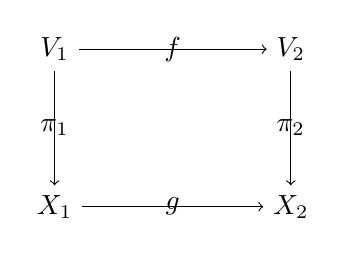
\begin{tikzpicture}
		\node (lt) {$V_1$};
		\node (rt) at (3,0) {$V_2$};
		\node (lb) at (0,-2) {$X_1$};
		\node (rb) at (3,-2) {$X_2$};
		\draw[->] (lt) to node {$f$} (rt);
		\draw[->] (lb) to node {$g$} (rb);
		\draw[->] (lt) to node [swap] {$\pi_1$} (lb);
		\draw[->] (rt) to node {$\pi_2$} (rb);
		\end{tikzpicture}
	\end{center}
	commutes and $f$ is fiberwise linear. That is, for every $x\in X_1$ the restriction of $f$ onto $\pi_1^{-1}(x)$ is a linear map between the vector spaces $\pi_1^{-1}(x)$ and $\pi_2^{-1}(g(x))$.
\end{defi}

\begin{defi}[$G$\=/linearisation of a line bundle, \phantom{}{\cite[chapter 1.3]{git}}]
	Let $G$ be an affine algebraic group acting on an affine variety $X$. Let $\pi\colon L \rightarrow X$ be a line bundle over $X$. A \emph{$G$\=/linearisation of $L$} is a bundle isomorphism $(f,g)$ from the line bundle $G\times L$ to $L$ such that
	$$f\colon G\times L \longrightarrow L$$
	is an algebraic group action and
	\begin{center}
		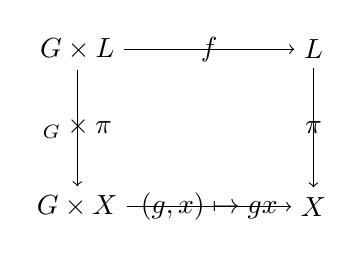
\begin{tikzpicture}
		\node (lt) {$G\times L$};
		\node (rt) at (3,0) {$L$};
		\node (lb) at (0,-2) {$G\times X$};
		\node (rb) at (3,-2) {$X$};
		\draw[->] (lt) to node {$f$} (rt);
		\draw[->] (lb) to node {$(g,x)\mapsto gx$} (rb);
		\draw[->] (lt) to node [swap] {$\id_G\times \pi$} (lb);
		\draw[->] (rt) to node {$\pi$} (rb);
		\end{tikzpicture}
	\end{center}
	commutes. A \emph{$G$\=/linearised line bundle} is a line bundle $L$ together with a  $G$\=/linearisation of $L$.
\end{defi}

\begin{remark}
	The tensor product $L_1 \otimes L_2$ of $G$\=/linearised line bundles $L_1$ and $L_2$ over $X$ with $G$\=/linearisations $f_1$, $f_2$ is the $G$\=/linearised line bundle that is obtained by taking the tensor product on the fibers. Its group action is given by $f_1 \otimes f_2$. Note that $L_1^{\otimes n}$ is isomorphic to the line bundle $L_1$ with the $G$\=/linearisation
	$$G\times L_1 \longrightarrow L_1,\quad (g, \ell) \mapsto f(g^n, \ell)$$
\end{remark}

\begin{remark}[Group action on sections, \phantom{}{\cite[Remark 1.7]{git_equivalence}}]
	Let $L$ be a $G$\=/linearised line bundle over $X$. For each $G$\=/invariant open subset $U\subseteq X$ we obtain a group action of $G$ on the space $\Gamma(U,L)$ of sections of over $U$ by setting
	$$g\cdot s(x) \defeq g\cdot(s(g^{-1}x)).$$
	The identity and compatibility axioms are verified easily. We check that $g\cdot s$ again is a section in $\Gamma(U,L)$. It is well defined on $U$ since we have $g^{-1}x\in U$ for all $g\in G$, $x\in U$. Clearly, $g\cdot s$ is the composition of morphisms and thus a morphism itself.
	
	The subspace of $G$\=/invariant sections of $L$ over $U$ is denoted by $\Gamma(U,L)^G$.
	\index{GammaULG@$\Gamma(U,L)^G$}%
\end{remark}

Now we are ready to describe the construction of semistable and stable points in accordance with \cite[Definition 1.7 \& 1.8]{git}. Note that for us, stable points mean properly stable points in the sense of Mumford.

\begin{defi}
	Let $L$ be a $G$\=/linearised, ample line bundle over $X$. A point $x\in X$ is called
	\begin{itemize}
		\item \emph{semistable} if there exists a $G$\=/invariant global section $s\in\Gamma(X,L^{\otimes n})^G$ for some $n\in\natural$ such that $s(x)\neq 0$, where $0$ is the origin in the fiber $\pi^{-1}(x)$.
		\item \emph{stable} if its stabiliser $G_x$ is finite and it is semistable via a global section $s$ such that all $G$\=/orbits in 
		$$X_s = X\setminus V(s) = \{p\in X\mid s(p) \neq 0 \}$$
		are closed.
	\end{itemize}
	The sets of semistable points and stable points are denoted by $X^{ss}(L)$ and $X^{s}(L)$ respectively.
\end{defi}

\begin{remark}
	By Mumford, the $G$\=/invariant set $X^{ss}(L)$ permits a good quotient $X^{ss}(L)\sslash G$, called \emph{GIT quotient}. It is the projective variety of the graded ring
	$$\bigoplus_{n\geq 0} \Gamma(X,L^{\otimes n})^G.$$
	If  $X^{s}(L)$ is non\=/empty, $X^{ss}(L)\sslash G$ is an almost geometric quotient with the restriction to $X^{s}(L)$ being a geometric quotient.
\end{remark}

\section{The GIT fan}

The set of semistable points $X^{ss}(L)$ and the corresponding GIT quotient depend on the choice of a $G$\=/linearised line bundle. As we will see in this section, we are able to parametrise all sets of semistable points arising from linearisations of the trivial line bundle by a special quasifan, called GIT fan, whose cones are in inclusion\=/reversing one\=/to\=/one correspondence. We assume that the group $G$ is an algebraic torus acting on an affine variety $X$. Note that the general case of arbitrary connected reductive groups $G$ may be reduced to the torus case, see \cite[Lemma 3.3]{git_via_cox_rings}. The concepts presented here originate from \cite[chapter 2]{git_equivalence}.

%An git-equivalence beyond the ample cone entlanghangeln (Kapitel 2)

%Notation: k-dim. Kegel: Fan^{(k)}

\section{Mori dream spaces, movable divisor classes?}